%%% template.tex
%%%
%%% This LaTeX source document can be used as the basis for your technical
%%% paper or abstract. Intentionally stripped of annotation, the parameters
%%% and commands should be adjusted for your particular paper - title, 
%%% author, article DOI, etc.
%%% The accompanying ``template.annotated.tex'' provides copious annotation
%%% for the commands and parameters found in the source document. (The code
%%% is identical in ``template.tex'' and ``template.annotated.tex.'')

\documentclass[annual]{acmsiggraph}
%\documentclass[review]{acmsiggraph}

\TOGonlineid{0000}
\TOGvolume{0}
\TOGnumber{0}
\TOGarticleDOI{1111111.2222222}
\TOGprojectURL{}
\TOGvideoURL{}
\TOGdataURL{}
\TOGcodeURL{}

% can I add packages at siggraph template?
\usepackage{amsfonts}
\usepackage[]{algorithm2e}
\usepackage{subcaption}

\DeclareMathOperator*{\argmax}{arg\,max}
\DeclareMathOperator*{\argmin}{arg\,min}

%\title{RegressAR: Object Pose Perspective Learning based on Feature Points Local Information and Decision Forest Regression for Augmented Reality}
\title{RegressAR: Learning Object Pose based on Feature Points Local Information for Augmented Reality}

%\author{paper\_ XXXX}
%\pdfauthor{paper_XXXX}


\author{Daniel M. Tokunaga\thanks{e-mail:dmtokunaga@acm.org}\\Escola Polit\'{e}cnica da USP
\and Munehiko Sato\thanks{e-mail:munehiko@acm.org}\\MIT Media Lab
\and Dan Raviv\thanks{e-mail:darav@mit.edu}\\MIT Media Lab
\and Ramesh Raskar\thanks{e-mail:raskar@media.mit.edu}\\MIT Media Lab
\and Romero Tori\thanks{e-mail:tori@acm.org}\\Escola Polit\'{e}cnica da USP}
\pdfauthor{Daniel M. Tokunaga}

\keywords{Augmented Reality, Pose Estimation, Regression Forest}

\begin{document}

 \teaser{
	\begin{subfigure}[c]{0.25\textwidth} \includegraphics[width=0.97\textwidth]{images/res_sig2016_1.png} \end{subfigure}%
	\begin{subfigure}[c]{0.25\textwidth} \includegraphics[width=0.97\textwidth]{images/res_sig2016_2.png} \end{subfigure}%
	\begin{subfigure}[c]{0.25\textwidth} \includegraphics[width=0.97\textwidth]{images/res_sig2016_3.png} \end{subfigure}%
	\begin{subfigure}[c]{0.25\textwidth} \includegraphics[width=0.97\textwidth]{images/res_sig2016_4.png} \end{subfigure}%	
   	\caption{Pose estimation based on our RegressAR approach.}
   	\label{img:teaser}
 }

\maketitle

\begin{abstract}

%Object pose estimation based on image information is one of key issues in augmented reality. However, conventional state-of-the-art non-iterative solve Perspective-$n$-Point approaches can be quite complex, once major solutions are based on the non-linear solvers. On the other hand, machine learning regression approaches have been applied for pose regression. Though, none of previous works achieved full pose. In this paper we propose RegressAR, a novel approach based on local information of feature points and decision forest regression, in order to fully estimate object poses. This machine learning based approach, yet simple, can provide comparable accuracy to state-of-the-art solutions. Also, for the global pose estimation of the object, we introduce a hybrid method between decision forest and RANSAC approach, named RF-RANSAC, in order to achieve better accuracy and performance. Although, we focus on planar objects pose estimation in this work, we show that our solution can be extended for other problems, such as 3D objects pose estimation. 

In this paper we propose RegressAR, a novel approach, based on local poses of image feature points and decision forest regression, in order to fully estimate the object pose. By applying regression training over scale and rotation invariant feature points appearances, we obtain estimations of the local rotations. These local rotations are, then, projected to global object information in order to find the full pose. Unlike other works of pose regression by machine learning presented in the literature, we are the very first to fully achieve, by machine learning, image feature points local rotation; and full 6 degrees-of-freedom object pose. This solution also avoids complex non-linear solvers, applied in several state-of-the-art non-iterative solve Perspective-$n$-Point approaches. We show that this machine learning based approach, yet simple, can provide comparable accuracy to state-of-the-art solutions.    
%
%In this paper we propose a novel approach for rigid pose estimation based on local image features as part of a learning system. We train a random forest over multiple scales and rotations obtaining a local signature invariant to such deformations, from which we infer the global pose. Comparing to other systems we do not need to solve complex non-linear systems, replacing that with a fast and robust approach showing comparable results and dramatically lower real-time calculation demands.

\end{abstract}

\begin{CRcatlist}
  \CRcat{H.5.1}{Information Interfaces and Presentation}{Multimedia Information Systems}{Artificial, augmented, and virtual realities}
  \CRcat{I.4.8}{Image Processing and Computer Vision}{Scene Analysis};
\end{CRcatlist}

\keywordlist

\TOGlinkslist

\copyrightspace

\section{Introduction}
\label{sec:intro}

% for AR! -> why object pose? 
% complexity of other methods  
% On the other hand, methods of machine learing based poses.

In the past years, a number of applications and ideas for augmented reality (AR) has been developed \cite{Benko:2014,Krevelen:2010}. However, linking a physical real objects with virtual information is still one central aspect on AR \cite{Krevelen:2010}. Usage of real objects as link to virtual contents is not only limited to visual augmentation \cite{Comport:2006}, but also with tactile sensations \cite{Bau:2012}, as methods of input \cite{Heun:2013}, or even output  \cite{Leithinger:2014}. And one central issue related to the visual augmentation is the spatial registration of these objects, or in other words, the estimation of the objects poses. 

Conventional methods for pose estimation with color images are often based on the correlation of known three-dimensional (3D) points to observed two-dimensional (2D) points. This correlation is known as perspective-$n$-points (P-$n$-P) problem \cite{Fischler:1981}. However, several solutions of this problem are based on complex non-linear equations solvers \cite{Lepetit:2009}. 

Also, in order to obtain this point correlation, feature points detection and matching \cite{Lowe:1999,Bay:2008} are applied in several P-$n$-P works \cite{Lowe:1999}. These feature points can give rich information, which could be used at the estimation process, however in several P-$n$-P approaches, these information are thrown away, where feature points are simplified as a single point in the space. 

%% change-> more ML with local + show a illsutration or explanation that is hard to overcome between 2DoF to 3DoF -> similarities that appear across the views. more explain.
On the other hand, works such as presented by Fenzi et al. \cite{Fenzi:2013}, explore machine learning regression approaches in order to learn the object pose, by the perspective distortion of these feature points; gathering more local information from each point. Despite that, they do not enable full pose estimation of the object.  

%% take off RF-RNASAC-> already applied in Brachmann works -> different-> but... -> so RegressAR is all now. No RF-RANSAC.  
%In this work, we address this full object pose estimation with our novel full pose estimation approach, named RegressAR, which applies regression forest \cite{Criminisi:Book} over the feature points appearance changes, in order to locally learn the perspective changes. Additionally, we introduce a novel hybrid method between regression forest and RANSAC approaches \cite{Fischler:1981}, named RF-RANSAC, to reach the object pose by this approach. In this method, we explore the prior information of the scene in order to refine the regression value returned by the regression forest. Here, we focus on planar object pose estimation, evaluating our method in comparison to state-of-art P-$n$-P method. Yet, we also show that our methods could be extended to 3D rigid object at the section \ref{subsec:results:other}.   

In this work, we address this full object pose estimation with our novel full pose estimation approach, named RegressAR, which applies regression forest \cite{Criminisi:Book} over the feature points appearance changes, in order to locally learn the perspective changes. This regression can provide us local rotations of each feature point, rich information that can be used in several conditions, such as in deformation estimation \cite{Tokunaga:2015,Rendl:2014}; that are not explored in conventional pose estimation works. 

After that, we explore the prior information of the scene in order to refine the regression value returned by the regression forest combined with RANSAC method. Here, we focus on planar object pose estimation, evaluating our method in comparison to state-of-art P-$n$-P method. Yet, we also show that our methods could be extended to 3D rigid object or deformable objects, at the section \ref{subsec:results:other}.   

Our main contribution in this work is our RegressAR approach itself, which can be a simple, yet accurate, alternative for AR systems. For the best of our knowledge, we are the very first to address this full pose of the object based on feature points local poses and machine learning approach. Thus, not needing to solve complex non-linear systems, replacing that with a fast and robust approach showing comparable results and dramatically lower real-time calculation demands.
%; unlike previous works that estimate only few degrees-of-freedom or are based only on points position information, not exploring the local poses.  
%The RF-RANSAC method is also another key contribution of this work.

In the next section we will present related works for object pose estimation. In section \ref{sec:poseMethod}, we present our RegressAR approach itself. Our obtained results are presented in section \ref{sec:results}, as well as its evaluation, in \ref{subsec:results:evaluation}, and extensions, \ref{subsec:results:other}. Finally we discuss our approach and its results in section \ref{sec:discussion}; and show our conclusion and future works in \ref{sec:conclusion}.


\section{Related Works}
\label{sec:relatedWorks}

Object pose estimation and tracking is one of key approaches in AR in order to obtain the spatial registration. This is achieved in several works by methods that solve the problem of Perspective-$n$-Points (PnP). Works such as \cite{Lu:2000,Lowe:1991} address this problem with iterative methods. Although these methods achieve good accuracy, they normally lack on computational performance \cite{Lepetit:2009}. 

Works such as \cite{Lepetit:2009,Li:2012} approach the solve P-$n$-P by noniterative methods. Li et al.\shortcite{Li:2012} address the PnP problem by minimizing several equations of 4th order polynomial, leading to solvers of 7th order, in order to obtain the rotation matrix first, to then obtain the translation matrix. Lepetit et al. \shortcite{Lepetit:2009}, on the other hand, address the PnP problem by expressing PnP to a weighted sum of 4 control points, and optimizing the 4th order polynomial using iterative Guass-Newton scheme. As we can see, all of these methods lay at the two points constrain in order to estimate the depth of the points, which, leads to complex non-linear polynomial solving problems, as pointed by \cite{Kukelova:2008}.     

%% machine learning + RGB -> murase + (lepetit class + other discrete) -> descrete 
%% RGB based more -> Torki, Gu, HoG baseds,  Fenzi, -> all not with 6DoF -> show in intro that is hard; explanation that is hard to overcome between 2DoF to 3DoF -> similarities that appear across the views. + no explict local.  also -> Hara and Shimizu
%% RGB-D based -> good results 6DoF and also local, similar to us Brachmann->RANSAC+RF (specially shotton:2013, Brachmann, Krull, and tajen?2015) -> rely on depth
%% our works is the only with continuous (not discrete as somes) 6DoF + Local rotation. -> Fenzi:2015 similar to Fenzi:2013 approach + Brachmann:2014; + Pepik:2012; + Similar to Changchang . Also to Tokunaga:2015 local poses -> rely on RGB-D cameras too. 

On the other hand, machine learning based approaches had become largely explored in pose estimation of known objects. Those approaches have the advantage of avoiding complex non-linear solving problems. Murase and Nayar \shortcite{Murase:1993} apply an eigen space analysis in order to learn the object poses and illumination changing. Then, works such as \cite{Lepetit:2009,Pepik:2012,Gu:2010} also applied machine learning for training the object pose across its appearances. However, such works inherently deal with discretized views. 

\cite{Torki:2011,He:2014,Hara:2014,Shimizu:2014,Zhen:2015} learn the object appearance across views in order to obtain continuous pose. Though, such approaches do not achieve full 6 DoF pose, neither the local pose of the feature points.%Specially HoG features based works can not directly returns full pose, once HoG features are not directly scale and rotation invariant.            
	
Besides that, works such as \cite{Shotton:2013,Brachmann:2014,Tejani:2014} also apply machine learning for full object pose estimation, despite based on depth and image information (RGB-D). In special, \cite{Tejani:2014} is similar to our approach, once authors train the local pose of the object, for each pixel. Also, all of those works apply random forest for pose estimation, as in our approach.  

Partial local information of pose also can be estimated in \cite{Fenzi:2013}, which apply regression based only on the feature points local appearance, and \cite{Pepik:2012}, which apply deformable part model with HoG features. However, none of the works based on machine learning presented here achieve full 6 DoF object pose, nor local rotation. Although some works propose that full rotation can be achieved by simply extending its method; this extension is not easy, due to similarities in appearance of feature points such as presented in \ref{img:diffL2}, specially to feature points that does not have rotation invariance. 

\begin{figure}[h]
\center
\begin{subfigure}{0.5\columnwidth} \center \includegraphics[width=0.9\textwidth]{images/L2dists_psi_phi_changes_30_img.png} 
\caption{3D view} 
\label{img:diffL2:3D}
\end{subfigure}%
\begin{subfigure}{0.5\columnwidth} \center \includegraphics[width=0.9\textwidth]{images/L2dists_psi_phi_changes_30_img_top.png} 
\caption{top view}
\label{img:diffL2:top}
\end{subfigure}%
\caption{L2 distances between feature points views with fixed $\theta$, and varying $\phi$, $\psi$ values of camera. $0$ valued distance in the graph is the reference view. It is possible to observe the similarity which appears all across different $\psi$ and $\phi$, making the extension of 2DoF rotation regression (fixed $\psi$) to 3DoF rotation non-trivial.}
\label{img:diffL2}
\end{figure}

Our RF-RANSAC method (section \ref{subsec:poseMethod:rfRANSAC}) is also similar to \cite{Brachmann:2014}, where regression forest method is combined with RANSAC method. Local feature points poses are also explored by \cite{Tokunaga:2015} for rigid and deformable object pose estimation. Despite those similarities, both works are based on RGB-D information, not being able to obtain local pose with only RGB images. Finally, \cite{Wu:2008} also shares similarities with our work, in the meaning that they also rely on local appearance changes for feature point matching; though, the final object pose is calculated with conventional RANSAC approach, also simplifying the local information to a simple point in space, and not achieving local rotation.    

%% img of different psi-theta

%%% change from here. 
%On the other hand, \cite{Torki:2011,Fenzi:2013,Fanelli:2011,Shotton:2011} presents another approach for pose estimation based on pattern matching of the object in different poses. Fanelli et al.\shortcite{Fanelli:2011} and Shotton and et al.\shortcite{Shotton:2011} presents the regression of body parts based on random forests. Shotton et al. additionally presents the hi-performance that decision forests can reach using GPU processing. \shortcite{Fanelli:2011} train decision forest directly to obtain the pose of the object, similarly to our approach. However, both works rely on depth maps for the estimation.
%
%Works such as \cite{Torki:2011}, \cite{Fenzi:2013} and \cite{} presents approaches based on analysis of near surrounding of feature points in color images in order to pose estimate rigid objects. In \cite{Torki:2011}, authors present a Kernel-based regression, and \shortcite{Fenzi:2013}, takes a n Nearest Neighbor approach in order to estimate the pose. Our work is more similar to \shortcite{Torki:2011} and \shortcite{Fenzi:2013} approaches of pose estimation. However, both methods only extract one or two dimensional pose of the objects. 
%% ??? 
%\cite{} also present an approach based on machine learning for pose estimation. Although authors present a possibility to find full transformation, they rely on the 2D image position of all the feature points and do not consider image similarities of the object when exposed to full affine transformations (?? as shown in figure \ref{???}); similarly to \cite{Muller:1993}. Thus, not obtaining full pose of the objects nor local rotation of each feature point.  
%% shapes-from-texture?
%Our work is similar to \cite{Lepetit:2006}, where decision forests are used in combination of the appearance changes around feature points across views. However, Lepetit and Fua \shortcite{Lepetit:2006} focus on keypoints classifications, not obtaining continuous object pose. Also, our work is similar to \cite{Tokunaga:2015}, where local poses are estimated in order to find the final object pose; however, in this work the authors are based on color image and also depth maps to find the local poses. Unlike all previous approaches, we address in this work the full pose estimation of objects; based only on color image patches of each feature points to extract their local poses using machine learning approaches.
%%%%




\section{Pose Estimation Method}
\label{sec:poseMethod}

\begin{figure*}[t]
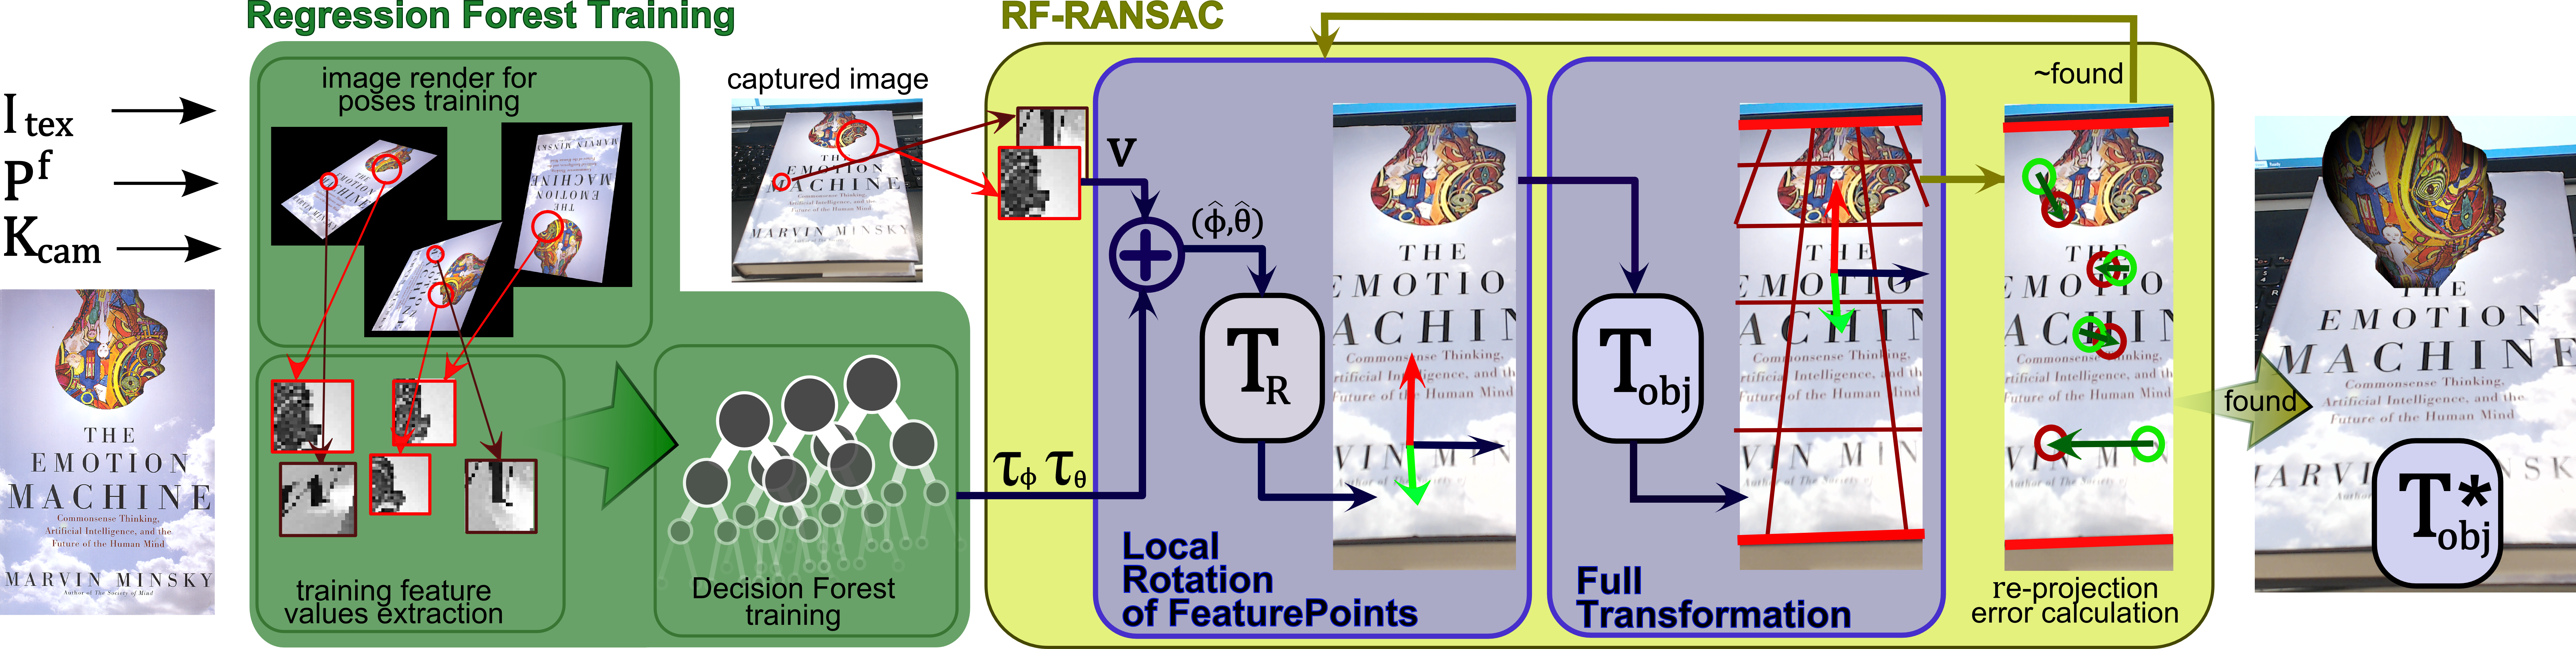
\includegraphics[width =\textwidth]{images/infoFlow.png}
\caption{Information flow of our approach.}
\label{img:inforFlow}
\end{figure*}
	
	
%% talk about similarities with other works across here also?

In this section we present our RegressAR approach for object pose estimation. The main idea behind our approach is to explore machine learning methods to learn the perspective changes based on appearance changes around detected features in order to estimate the object pose. First, in order to achieve our pose estimation, we consider three different Euclidian coordinate spaces. The image space $I$, which are the two-dimensional space of captured images; and world coordinates $w$, the three-dimensional space of the scene where object pose needs to be calculated. At last, pre-captured  information about the object are hold in $o$, the three-dimensional coordinate space of the original planar object model. 

From this point of this work, we denote that variables with a uppercase $I$, such as $x^I$, denotes that are in image space; variables with $o$, the original coordinates of the captured object; and $w$, the new scene world coordinate. Also, points with upper case $H$ denotes the homogeneous coordinates of the projected point, i.e., $\mathbf{p}^H = \mathbf{p}^w/z = [x/z, y/z, 1]^\top$. 

For perspectives changes training, we assume that the object is locally rigid and planar around the feature points. This assumption is always true for planar objects, but also could be extended for different types of object, such as 3D rigid objects \cite{Lepetit:2005} or locally rigid deformable objects, making our approach for these type of object as same as planar objects. Also, we assume that object surface texture $I_{tex}$, as well as, that the camera projection matrix $\mathbf{K}_{cam}$ are known. 
%Moreover, we consider that the unfolding model of the object surface to a planar surface is known. This unfolding model is composed by the function that maps any transformation in the object space to the unfolded texture space, $f_u(T^o) = T^t$; and its inverse $f_u^{-1} = f_f(T^t) = T^o$, that maps any transformation in texture space to original space, are known. This functions are similar to UV mapping algorithms \cite{}, or unfolding methods such as \cite{}. With these functions, we can unfold the object texture to a plane and process all the feature points in the model as a planar object.     

Another assumption is that the $\theta$ and $\phi$ values of the camera are independent for the deformation of the projected surface to the image. This means that we can estimate each value independently of the other, as in \cite{Fenzi:2013}. Finally, we assume that the set of rotation and scale invariant feature points $P^f = \{ p^f_0, \ldots, p^f_n \}$, such as SIFT \cite{Lowe:1999} or SURF \cite{Bay:2008}, spread across the object surface texture are known. Each feature point $p^f_i$ contains a set of information $p^f_i = \{ \mathbf{p}^o_i, \mathbf{o}^o_i, dsc_i \}$, where, $\mathbf{p}^o_i$ is the position of the point and $\mathbf{o}^o_i$, the orientation vector, both in the original object space; and $dsc_i$, the feature point descriptor. 

Our camera model is similar to ASIFT work \cite{Morel:2009}, which can produce all the affine transformations for a planar object as presented by authors. Figure \ref{img:cameraModel} presents our applied camera model. Note that $\psi$ rotation is related to image space rotation. Furthermore, once feature points that we are applying for our method are rotation invariant \cite{Bay:2008}, our training data can be $\psi$ invariant, needing to train only $\theta$ and $\phi$ values per feature point deformations. At subsection \ref{subsec:poseMethod:rotMat}, we show more details how to proceed this $\psi$-invariant training.   

% img of camera model   
\begin{figure}[h]

\center
\begin{subfigure}[c]{0.4\columnwidth} \center \includegraphics[width=0.9\textwidth]{images/camModel_objCenter.png} 
\caption{object centered coordinates} 
\label{img:cameraModel:obj}
\end{subfigure}%
\begin{subfigure}[c]{0.6\columnwidth} \center \includegraphics[width=0.9\textwidth]{images/camModel_camCenter.png} 
\caption{camera centered coordinates}
\label{img:cameraModel:cam}
\end{subfigure}%
\caption{Camera pose models for regression. Camera model in figure \ref{img:cameraModel:obj} is used in the training part, and figure \ref{img:cameraModel:cam}, for the pose estimation part. }
\label{img:cameraModel}
\end{figure}

Our entire RegressAR approach is separated in four parts, 
\begin{enumerate}
  \item \textbf{regression forest training}: which generates the regression forest from samples of the object feature in several poses;
  \item \textbf{local rotation pose estimation}: which estimates the rotation pose of the feature point based on the observed feature point local information;
  \item \textbf{full transformation matrix estimation}: estimates the translation value of the feature points by using a second point; 
  \item \textbf{Random Forest Random Sample Consensus (RF-RANSAC)}: estimates the global object pose by combining decision forest and RANSAC approaches.
\end{enumerate}
Figure \ref{img:inforFlow} illustrates the entire approach information flow.

\subsection{Regression Forest Training}
\label{subsec:poseMethod:rfTrain}


The goal here is to train the appearance information around feature points across different $\theta$ and $\phi$ values for the camera position regression, based on the rotation invariant feature points. First, we use a synthetic approach to generate samples for training, similarly to \cite{Morel:2009} and \cite{Criminisi:Book}. We render the object surface texture $\mathbf{I}_{tex}$ as planar object with different camera poses, using the same camera projection matrix $\mathbf{K}_{cam}$ of the scene capturing camera. 

In each rendered image, we convert the color pixel values to brightness values and process a conventional feature matching algorithm \cite{Bay:2008} in order to find the matching feature points in the new image. Then, for each matched features point, we extract the feature point training feature values $\mathbf{v}_{tr}$.   

This training features extraction is done by first extracting a small square image patch around the feature points. This image patch has a length of $l_{diag}$, which is based on the scale factor of the feature point, $s_{ft}$. Therefore, our transformation in the image space is extracted with size $l_{diag} = n_{pix}s_{ft}\sqrt{2}$. Where, $n_{pix}$ is the number of the pixels to be extracted.

%Once, feature points in SURF and SIFT are blob like features, changing $n_{pix}$ greater then the conventional value used to analyze the interest point, makes the $\theta$ and $\phi$ regression better, although, it can make the patch capture also the background.     

Then, this  image patch is rotated using the inverse of orientation value $o_{ft}$ of the feature point. This creates an image patch that always is oriented to the major orientation of the feature point, despite the $\psi$ value of the frame. Then, this new patch is cropped to fit $l_{feat} = n_{pix}s_{ft}$, and rescaled to the size of the training samples feature $l_{ft}$. 

This image patch is converted to an array of size $l_{ft}^2$, in order to obtain training feature values $\mathbf{v}_{tr} \in \mathbb{R}^{l_{ft}^2}$.  At last, the feature values are normalized to a interval of $[0,1]$, in order to make the feature less affected by brightness changes. Figure \ref{img:imgPatchSearch} illustrates this entire process. 
%
%This process is similar to applying a 2D transformation
%\begin{equation}
%\mathbf{T}^I = \mathbf{T}_t^I \cdot \mathbf{T}_{rot}^I \cdot \mathbf{T}_{s}^I 
%\label{eq:2dImgPatch}
%\end{equation}
%to the feature values grid. Where, $\mathbf{T}_t^I$ is a 2D translation matrix to the position $p_x^I$ and $p_y^I$ of the feature point; $\mathbf{T}_r^I$ is a 2D rotation matrix of angle $o$, the major orientation returned by the feature point; and finally, $\mathbf{T}_s^I$, a scale matrix of scaling factor $(s_{ft}\, n_{pix})$. Capturing the pixels within $[(-s_{tr}/2, -s_{tr}/2), \ldots, (s_{tr}/2, -s_{tr}/2), \ldots, (s_{tr}/2, s_{tr}/2) ]$ of the grid, will return the same samples training features values. Figure \ref{img:imgPatchSearch} also illustrates this process. 
%Figure \ref{img:featChanges} illustrates the changes of the first $15$ values of the patch across changes in $\theta$ and $\phi$.
%

% img: patch capture -> small patch -> rotated -> rescaled -> normalized
\begin{figure}[h]
\center
\includegraphics[width =\columnwidth]{images/patchExtraction_misky.png}
\caption{Near feature point image patch extraction for training feature value $\mathbf{v}$ extraction by image processing.}
\label{img:imgPatchSearch}
\end{figure}
%
%\begin{figure}[h]
%\center
%\begin{subfigure}[c]{0.5\columnwidth} \center \includegraphics[width=0.98\textwidth]{images/thetaChanges.png} 
%\caption{feature values changes across $\theta$ changes with fixed $\phi$.} 
%\label{img:featChanges:theta}
%\end{subfigure}%
%\begin{subfigure}[c]{0.5\columnwidth} \center \includegraphics[width=0.98\textwidth]{images/phiChanges.png} 
%\caption{feature values changes across $\phi$ changes with fixed $\theta$.}
%\label{img:featChanges:phi}
%\end{subfigure}%
%\caption{Training features values changes across $\theta$ and $\phi$ values, each one with different feature points. Illustrating the changes of pixel color across poses. Moreover, the difference between different feature points.}
%\label{img:featChanges}
%\end{figure}


% In order to train the affine transformation related changes, we synthetically generate the object texture surface in several poses, similarly to \cite{}. 
In order to achieve the well spread representative sampling data for the training, we generate several random samples with different $\theta$ values, within $[\pi/2, \ldots ,0]$, and $\phi$, within $[0,\ldots,2\pi]$. In order to train small errors created by rotation and scale values, we also use random $\psi$, $x$, $y$ and $z$ values. Furthermore, we add a gaussian noise of mean $0$ and several standard deviations $\sigma$s, in order to make our regression results more robust to image noises. Figure \ref{img:samplesExamples} illustrates part of the images and sample patch used at the training. Note that variations are more strong when $\theta$ is higher, once the image plane is less orthogonal to the camera.  

% img: samples and patch samples?
\begin{figure}[h]
\includegraphics[width =\columnwidth]{images/patchesAcross.png}
\caption{Training feature values with different object poses across $\theta$ and $\phi$ values. Y axis shows changes in $\theta$ varying from $90$ degrees to $35$ degrees. X, across $\phi$ changes from $0$ to $360$ degrees.}
\label{img:samplesExamples}
\end{figure}

For the training itself, we apply a regression forest approach, due to its capability of generating fast regression results for real-time applications, among other advantages such as described in \cite{Criminisi:Book}. The decision forest approach is based on the multiple decision tree training\cite{Criminisi:Book}. Here, we generate $n_{\tau}$ decision trees for each extracted feature point $f$.  


Once we assumed that $\theta$ and $\phi$ are independent, we can generate a set of $n_{\tau}$ trees, $\tau_{(\theta,f)}$, for the $\theta$ value, and $n_{\phi}$ trees, $\tau_{(\phi,f)}$ for $\phi$ values. However, decision forest also can be a memory expensive method, and training all the feature points of the object can rapidly increase the memory consumption. In order to avoid this problem, we can train only a set of $P^{rf}$ perspective robust feature point within $P^{f}$. Here, we select $P^{rf}$ as the $n_{rf}$ feature points that most appear across different rendered images.    

Other feature points within $P^{f}$, are still used as verification points at the calculation process, as described in section \ref{subsec:poseMethod:rfRANSAC}. At the end of this point, we have generated several feature points $P^{rf}$, each, attached with several regression trees $\tau_{(\theta, f)}$, $\tau_{(\phi, f)}$, where $P^{rf} \in P^{f}$, based the samples images. 
%In the next section we will present the rotation matrix estimation based on local information of each matched feature point in a new frame.   

% talk of how they train trees and the multiple trees.   and that \theta and \phi are independent trees! and that we dont need to train all the feature point with trees!! we can do by a part, but use all for the next steps.


\subsection{Local Rotation Matrix of Feature Points}
\label{subsec:poseMethod:rotMat}

In order to process the pose estimation itself in a newly observed frame $I_{obs}$, we first proceed a feature matching algorithm to find the matching feature points, $\mathbf{P}^I_{m}$, between $p^I_{obs}$ and $P_{f}$. Then, we capture the image patch as in section \ref{subsec:poseMethod:rfTrain}, for each matched point $f$ within $P_{rf}$, points that has a regression forest associated. 


We then extract the feature values vector $\mathbf{v}^{t}_{f}$, of each image patch. By applying a regression with the forest and feature vector, each regression tree will return a prediction of $\hat{\theta}$ and $\hat{\phi}$. Based on the returned values of $\hat{\theta}$ and $\hat{\phi}$, we first calculate the rotation matrix. 

This rotation transformation is calculated as 
\begin{equation}
\mathbf{T}_{r} = \mathbf{T}_{\psi}\cdot\mathbf{T}_{\phi}\cdot \mathbf{T}_{\theta}, 
\label{eq:rotTrans}
\end{equation}
where $\mathbf{T}_{\theta}$ is a rotation around the $x$-axis with $\theta$; $\mathbf{T}_{\phi}$, around $y$-axis with $\phi$ and finally, $\mathbf{T}_{\psi}$, a rotation around the direction of the camera, $(-z)$-axis. However, once the regression is $\psi$-invariant, now we need to re-estimate the $\psi$ value for this new frame. This can be done by using a second known vector $\vec{v}_{\psi}$. 

This $\vec{v}_{\psi}$ can be calculated by a second matched 2D point, or also by the extracted orientation $o$ of the feature point. Using the orientation of the feature point itself enable us to calculate the rotation matrix of the object by only information from the feature point. This characteristic enable us obtain other unique results, as discussed at section \ref{sec:discussion}. When using the orientation of the feature point itself, we set $\vec{v}_{\psi}^o = \vec{o}_{f}^o$ and $\vec{v}_{\psi}^I = \vec{o}_{f}^I$, where $\vec{o}_{f}^I$ is the observed vector calculated by orientation $o$ returned by the feature point, $\vec{o}_{f}^I = [cos(o), sin(o)]$.  

However, small errors can occur at the feature point orientation. These errors can lead in global pose error of the object. Using a second point as $\vec{\mathbf{v}}_{\psi}$, gives us more stable results. In this case, we set $\vec{v}_{\psi}^o$ to be the unit vector with same direction as $\mathbf{p}_{f}^o - \mathbf{p}_{2}^o$ and $\vec{v}_{\psi}^I$ unit vector with direction $p_{f}^I - p^I_{2}$, where $\mathbf{p}_{2}^o$ is the original 3D location of the feature point and $p_{2}^2$, the observed location of the second point at the image space. 

After calculating $\vec{v}_{\psi}^I$ and $\vec{v}_{\psi}^o$, we calculate the final rotation matrix by finding $\hat{\psi}$ that matches the captured $\vec{v}_{\psi}^I$ with transformed $\vec{v}_{\psi}^o$, as illustrated by figure \ref{img:psiCalc}. Initially, $\vec{\mathbf{v}}^w(\hat{\psi})$ is calculated to be the final position of the transformed $\vec{\mathbf{v}}^o$ as
\begin{equation}
\vec{\mathbf{v}}^w(\hat{\psi}) = \mathbf{T}(\hat{\psi})\mathbf{T}_{\hat{\phi}}\mathbf{T}_{\hat{\theta}}\cdot \vec{\mathbf{v}}_{\psi}^o. 
\end{equation}
Where, $\mathbf{T}_{\hat{\phi}}$ and $\mathbf{T}_{\hat{\theta}}$ are the transformation matrices calculated by returned $\hat{\theta}$ and $\hat{\phi}$, and $\mathbf{T}(\hat{\psi})$ calculated with the unknown variable $\hat{\psi}$.
 
% img with the relation of $\vec{v}_{\psi}$ and projected $\vec{v}_{\psi}$ to the image plane
\begin{figure}[h]
\center
\includegraphics[width = 0.8\columnwidth]{images/rotCalc.png}
\caption{$\psi$ calculation model.}
\label{img:psiCalc}
\end{figure}
%
%Once $\vec{\mathbf{v}}^w(\hat{\psi})$ projected to the image plane, defined by $\hat{\mathbf{X}}$ and $\hat{\mathbf{Y}}$ axis, has same direction as $\vec{\mathbf{v}}_{\psi}^{obs}$; we have that
%\begin{equation}
%\begin{bmatrix}
%	\hat{\mathbf{X}} \cdot \vec{\mathbf{v}}^w(\hat{\psi})  \\[0.3em]
%	\hat{\mathbf{Y}} \cdot \vec{\mathbf{v}}^w(\hat{\psi})
%\end{bmatrix} 
%\propto \vec{v}_{\psi}^{obs}
%\label{eq:psi:idea}
%\end{equation}
%. Where, $\vec{v}_{\psi}^{obs}$ is observed $\vec{v}_{\psi}^I$ projected to the world coordinates as % need? instead of giving obs name, cane be I? 
%\begin{equation}
%\vec{\mathbf{v}}_{\psi}^{obs} = (z_{i}\mathbf{K}_{cam}^{-1}\mathbf{p}^o - z_{i}\mathbf{K}_{cam}^{-1}(\mathbf{p}^o + \vec{\mathbf{v}}_{\psi}^I))
%\end{equation}


Once $\vec{\mathbf{v}}^w(\hat{\psi})$ projected to the image plane, defined by $\hat{\mathbf{X}}$ and $\hat{\mathbf{Y}}$ axis, has same direction as $\vec{\mathbf{v}}_{\psi}^{obs}$. Where, $\vec{v}_{\psi}^{obs}$ is observed $\vec{v}_{\psi}^I$, projected to the world coordinates as 
\begin{equation}
\vec{\mathbf{v}}_{\psi}^{obs} = (z_{i}\mathbf{K}_{cam}^{-1}\mathbf{p}^o - z_{i}\mathbf{K}_{cam}^{-1}(\mathbf{p}^o + \vec{\mathbf{v}}_{\psi}^I)).
\end{equation}
Once, they must have same direction, we can calculate $\hat{\psi}$ by
\begin{equation}
\frac{ \vec{\mathbf{v}}_{\psi}^{obs}[x]}{ \vec{\mathbf{v}}_{\psi}^{obs}[y]} = \frac{\hat{\mathbf{X}} \cdot \vec{\mathbf{v}}^w(\hat{\psi})}{\hat{\mathbf{Y}} \cdot \vec{\mathbf{v}}^w(\hat{\psi})}.
\label{eq:psiCalc}
\end{equation}


By \eqref{eq:psiCalc}, we can find $\hat{\psi}$, that rotates the feature point to the same direction to $\vec{v}_{\psi}^I$. Therefore, being able to calculate the rotation matrix of the local feature point $\mathbf{T}_r$ by \eqref{eq:rotTrans}.

%% image space correction?  image showing the difference? 

% show local rotation results img?

\subsection{Full Transformation Matrix Estimation}
\label{subsec:poseMethod:fullT}
% show local rotation 

%%% paragraphs %%%
% after calculating the three rotations values of the feature point .... global pose..... 
	% however, as shown at figure \ref{trees return}, ....	

After calculating the rotation matrix, we now estimate the full transformation matrix of each feature point. In order to estimate the full transformation of the object, we need to estimate the $z$ position of the feature point. This is done by, again, applying the information of a second point $\mathbf{p}_{2}$. This calculation of $z$ is done by fitting the distance between two rotated point to the observed distance. 

%This calculation of $z$ is done by fitting the distance between two rotated point to the observed distance. Figure \ref{img:zCalc} illustrates this calculation process.  

%\begin{figure}[h]
%\center
%\includegraphics[width = 0.8\columnwidth]{images/zCalc.png}
%\caption{$z$ calculation model in order to estimate the translation of the object pose.}
%\label{img:zCalc}
%\end{figure}

First, we consider that the global position of a second point of the object $\mathbf{p}_2^w$, can be calculated by the sum of the position of the first observed feature point $\mathbf{p}_f^w$ and the rotated vector between both original positions $\mathbf{p}^o_2$ and  $\mathbf{p}^o_f$. As
\begin{equation}
\mathbf{p}_2^w = \mathbf{p}_f^w + \mathbf{T}_{r}\cdot(\mathbf{p}^o_2 - \mathbf{p}^o_f),
\label{eq:p2w}
\end{equation}
where, the global position of the observed feature point can be estimated by 
\begin{equation}
\mathbf{p}_f^w = z^w\mathbf{K}^{-1}_{cam}p^I_f.
\label{eq:pfproj}
\end{equation}
Note that here, the only unknown variable is $z^w$, $z$ coordinate of $\mathbf{p}_{f}^w$. Also, note that this is true only for pair of points with rigid transformation, where the distance between both point does not change across time.   

Then, by combining \eqref{eq:p2w} and \eqref{eq:pfproj}, and projecting the second point to the image plane we have
\begin{equation}
p_2^I = \mathbf{K}_{cam}(z^w \mathbf{K}^{-1}_{cam}\cdot p^I_1 + \mathbf{T}_{r}(\mathbf{p}^o_2 - \mathbf{p}^o_1))^H,
\label{eq:zCalc}
\end{equation} 	  
where $p_2^I$ is the image coordinates of the observed second point. By \eqref{eq:zCalc}, we can calculate the $z^w$ coordinate of the observed feature point global position. Finally object translation is given by $\mathbf{t} = z^wK^{-1}_{cam}p^I_1 - \mathbf{T}_r \mathbf{p}^o_1$. By combining the rotation transformation obtained in section \ref{subsec:poseMethod:rotMat} and the translation matrix $\mathbf{T}_t$ calculated using $\mathbf{t}$, we obtain the object full transformation $\mathbf{T}_{obj}$ by
\begin{equation}
\mathbf{T}_{obj} = \mathbf{T}_t\mathbf{T}_r.
\label{eq:Tobj}
\end{equation}
 

\subsection{Random Forest Random Sample Consensus}
\label{subsec:poseMethod:rfRANSAC}
% random forest bayesian model
% ?/results of theta and phi regression?
% ?per tree result to show that some really are good but mean (conventional model of forest is not good)?

	
%% paragraphs %%%%%

% the global pose can be calculated as.... but in this case we have the observations...... baies rule.....
% Furthermore, in order to achieve results faster, we have combined the Decision Forest with bservation approach with RANSAC....
% Initially, the full transformation of the object pose, based on a single feature and second 2D point, and prediction result of a single tree....
% Translation is calculated....
% As in RANSAC approaches, for rigid objects.....
	% however, differently from conventional decision forest....

For rigid object, one simple way to estimate the final object pose, based on the regression returned by several trees of several feature points, could be done by only taking the mean of returned $\hat{\theta}$ and $\hat{\phi}$, as conventional approaches \cite{Criminisi:Book}, and using the same calculation of section \ref{subsec:poseMethod:rotMat} and \ref{subsec:poseMethod:fullT}.

However, as illustrated at figure \ref{img:treeResults}, regressions returned by part of the trees has good accuracy, yet, other part has big errors around some values. In the first row of figure \ref{img:treeResults}, we present L1 norm errors returned by $20$ trees from one features values input. We can observe that, although $\theta$ returns good accuracy, $\phi$ regression has part of its trees with great errors. 

This result is confirmed by the confusion matrices at the second row of figure \ref{img:treeResults}. $\theta$ regression has a fall down in higher values, but this is caused by the fact that the image plane is less orthogonal to the camera direction. However, we also can observe that $\phi$ almost always have a second high probability peak, which creates wrong regression results.
	
\begin{figure}[h]
\begin{subfigure}[c]{0.5\columnwidth} \includegraphics[width=\textwidth]{images/eval_phiTrees_L1dist.png} \end{subfigure}%
\begin{subfigure}[c]{0.5\columnwidth} \includegraphics[width=\textwidth]{images/eval_thetaTrees_L1dist.png} \end{subfigure}\\%
\begin{subfigure}[c]{0.5\columnwidth} \includegraphics[width=\textwidth]{images/phi_map.png} \end{subfigure}%
\begin{subfigure}[c]{0.5\columnwidth} \includegraphics[width=\textwidth]{images/theta_map.png} \end{subfigure}%
\caption{ Trees regression accuracy evaluation. First row: Per tree returned value L1 error for one value. Showing that part of trees return accurate results; however others, return wrong values around certain value. Second row: confusion matrix evaluation with 1000 non-trained images; Y axis represents the ground truth value, and X axis, the predicted value. Also illustrating the errors in $\phi$ regression.}
\label{img:treeResults}
\end{figure}

This could happen because of similarities of the patch deformations in two different views. However, unlike conventional decision trees, where the regression value is calculated based on the input feature values $\mathbf{v}$ as  
\begin{equation}
p(\mathbf{T}_{obj}|\mathbf{v}) = \prod_{i} p_i(\mathbf{T}_{obj}|\mathbf{v}),
\label{eq:conventionalRF}
\end{equation}
here in this work, we have also other prior information about the object pose that could be used in order to refine the pose regression. 

One strong prior information are the distances between observed and reprojected 2D points of the feature points $\mathbf{p}^I_{m} = [(p^I_0, \mathbf{p}^f_j), \ldots, (p^I_n, \mathbf{p}^f_k)]$, such as used in many works of solve P-$n$-P problems \cite{Lepetit:2009,Li:2012}. These information also can be applied to the forest regression in order to improve the overall accuracy.

We inject this prior information at \eqref{eq:conventionalRF} by calculating
\begin{equation}
p(\mathbf{T}_{obj}|\mathbf{v}, \mathbf{p}^I_m) = \prod_{i} p_i(\mathbf{T}_{obj}|\mathbf{v}, \mathbf{p}^I_m).
\label{eq:RFprob:2Dpriori}
\end{equation}
By applying the Bayes rule, \eqref{eq:RFprob:2Dpriori} can be extended as
\begin{equation}
p(\mathbf{T}_{obj}|\mathbf{v}, \mathbf{p}^I_m) = \prod_{i} \frac{p_i(\mathbf{T}_{obj}|\mathbf{v})p_i(\mathbf{p}^I_m|\mathbf{T}_{obj},\mathbf{v})}{p_i(\mathbf{p}^I_m)}.
\label{eq:RFprob:bayes}
\end{equation}
Here $p_i(\mathbf{p}^I_m|\mathbf{T}_{obj},\mathbf{v})$ is the probability of finding the projected $\mathbf{p}^o$ to the image plane in $\mathbf{p}^I_m$ position by applying $\mathbf{T}_{obj}$. Once the re-projected positions $\mathbf{p}^I_m$ are independent of the feature values $\mathbf{v}$ used in regression, $p_i(\mathbf{p}^I_m|\mathbf{T}_{obj},\mathbf{v})$ can be simplified as $p_i(\mathbf{p}^I_m|\mathbf{T}_{obj})$. 

This reprojection probability $p_i(\mathbf{p}^I_m|\mathbf{T}_{obj})$ is inversely related to the sum of two-dimensional distance errors $\epsilon^{I}$ between the reprojected point, transformed by $\mathbf{T}_{obj}$, and observed point. This error can be calculated as
\begin{equation}
\epsilon^{I} = ||p^I_i - \mathbf{K}_{cam}(\mathbf{T}_{obj}\mathbf{p}^o_i)^H||.
\label{eq:epsilonI}
\end{equation}
Hence, as the distance $\epsilon$ increases, the probability $p_i(\mathbf{p}^I_m|\mathbf{T}_{obj})$ of $T_{obj}$ decreases; we can approximate $p_i(\mathbf{p}^I_m|\mathbf{T}_{obj})$ to be inversely proportional to $\epsilon^I$.


We now can rewrite equation \eqref{eq:RFprob:bayes} to estimate the best transformation $T_{obj}^*$ as 
\begin{equation}
\mathbf{T}_{obj}^* = \argmax \; p(\mathbf{T}(\theta, \phi)| \mathbf{v}, \mathbf{p}^I_m).
\label{eq:argmaxForest}
\end{equation}	
$T(\theta,\phi)$ can be calculated by the $\hat{\theta}$ returned by the trees $\tau^j_{(\theta,f)}$; and $\hat{\phi}$, by $\tau^k_{(\phi,f)}$, both from feature point $f$. We, also consider that the probability of the returned transformation from the trees $p_i(\mathbf{T}_{obj}|\mathbf{v})$, and the observed points $p_i(\mathbf{p}^I_m)$, are constant. 

Finally, we have that $p_i(\mathbf{p}^I_m|T(\theta_j,\phi_k))$ is inversely proportional to sum of the re-projection error $\epsilon$, as in \eqref{eq:epsilonI}, thus having
\begin{equation}
\begin{split}
\mathbf{T}_{obj}^* &\approx \argmin_{i,j,k} \sum_l \epsilon^I_{i,j,k} \\
&\approx \argmin_{i,j,k} \sum_l \| p^I_{l} - \mathbf{K}_{cam}(\mathbf{T}(\theta_{(j,i)}, \phi_{(k,i)})p^o_l )^H \|.
\end{split}
\label{eq:finalT}
\end{equation} 
By \eqref{eq:finalT}, we can calculate the final $\mathbf{T}_{obj}^*$ as the transformation that has least reprojection error calculated by all combinations of $\hat{\theta}$ and $\hat{\phi}$ returned from all the feature points $f$.     

However, calculating all the re-projections of the matched points, with all possible $\hat{\theta},\hat{\phi}$ trees regression of all feature points $f$ can be computationally heavy. In order to make this process faster for real-time applications such as in AR, we also propose here a hybrid approach between our pose regression forest with RANSAC method \cite{Morel:2009}, the Random Forest Random Sample Consensus (RF-RANSAC).  

In our RF-RANSAC approach, we combine the random sampling idea inside the decision forest. Thus, not only randomly sampling the observation nor features to be used, as a conventional approach, but also randomly sampling the trees within all the decision trees of all feature points. 

As in \cite{Morel:2009}, we first sample a subset $S1$ as a percentage $p_{s}$ of all matched feature points within $\mathbf{p}^I_{m}$ to use in the reprojection error calculation. Then, we randomly choose a matched feature point $p^f_i$ that has a decision forest attached in. 

We calculate the possible transformation $T_{obj}$ by extracting the regression feature values $\mathbf{v}_i$ of $p^f_i$ in the new image. We also randomly choose one $\theta$ regression tree $\tau_{(\theta,i)}^j$, and a $\tau_{(\phi,i)}^k$ for $\phi$, within in $p^f_i$ regression forest, in order to obtain $\hat{\theta}$ and $\hat{\phi}$ by $\mathbf{v}$. After this, we calculate the object transformation $\mathbf{T}_{obj}$ as in \ref{subsec:poseMethod:fullT}. 

The reprojection errors of the observed point and $\mathbf{T}_{obj}$ is calculated similar to \eqref{eq:epsilonI}, using $S1$. If the number of point that has $\epsilon^{I}$ smaller than distance threshold $d_{th}$, is greater than acceptance percentage $p_{th}$ of the subset, we accept $\mathbf{T}_{obj}$ as the object pose. Elsewhere, we keep re-estimating $\mathbf{T}_{obj}$ by using other random sample of feature point, $\theta$-tree and $\phi$-tree, while \eqref{eq:ransacDet} is not satisfied. Finally, if we not found a $\mathbf{T}_{obj}$ that satisfies \eqref{eq:ransacDet} within $n_{trial}$s; we then, set the object transformation $\mathbf{T}_{obj}$ as the transformation that had minimal error in the $n_{trials}$, as in \eqref{eq:finalT}. We illustrates the entire RF-RANSAC process at the algorithm \ref{alg:RF-RANSAC}.

% algorithm of the RF-RANSAC.    
%\begin{figure}[h]
\RestyleAlgo{boxruled}
\begin{algorithm}[h]
	\KwData{$P^f$; set of $\tau_{(\theta,f)}$ and $\tau_{(\phi,f)}$; $P_m^I$; $d_{th}$;  $p_{th}$; $p_{s}$ }
 	\KwResult{Full transformation matrix $T_{obj}$ of the rigid object}
 	%Set $n$ to $0$ and $found$ = $false$\;
 	\While{($found == false$) \& ($n < n_{trials}$) }{
  		Select random $p^f_i$ within $P^I_m$\;
  		Select random $\tau_{(\theta,i)}^j$ and $\tau_{(\phi,i)}^k$\;
  		Regress $\hat{\theta}^j$ and $\hat{\phi}^k$\;
  		Select random second point $\mathbf{p}_2^I$ and its original $\mathbf{p}_2^o$\;
  		Calculate $T_r$, as in \eqref{eq:rotTrans}, and $T_{obj}$, as in \eqref{eq:Tobj}\;
		Select a random set of points $S1$, by $p_{s}$\;  
		\ForAll{points within $S1$}{
			Calculate $\epsilon^I$
		}
		\eIf{$\#[ \epsilon^I < d_{th} ] < p_{th}\cdot p_{s} \cdot N$}{
			$found = true$\; 		
		}{
			\If{$\sum(\epsilon^I) < \epsilon_{min}$}{
				Storage current transformation $T_{obj}$ as minimal error transformation\;
				Update $\epsilon_{min} = \sum(\epsilon^I)$\;
			}
		}	
	
	}
 	\If{$fount \neq true$}{
		Use minimal error transformation as final $\mathbf{T}_{obj}$\; 	
	}
	Return found $T_{obj}$\; 	
\caption{RF-RANSAC algorithm}
\label{alg:RF-RANSAC}	
\end{algorithm}

\section{Results}
\label{sec:results}


We show case our RA results in figures \ref{img:resAR} and \ref{img:teaser}, calculated by our RegressAR pose estimation approach. Results showed in these figures were obtained by using SURF feature \cite{Bay:2008} as features points, with $20$ trees of $\tau_{\theta}$ and $\tau_{\phi}$ each, of $20$ different feature points. Other than these forest attached feature points, we also use $280$ feature points to help in the reproject error calculation and as second point for the rotation and translation calculation. In total, $300$ feature points are used for the matching. The observation distance threshold $d_{th}$ was set to $7$ pix, $S1$ subset percentage $p_{s}$ to be $60\%$ of entire observation, acceptance percentage $p_{th}$ as $80\%$, and $n_{trials}$ to be $100$.  

Moreover, we set as $n_{pix} = 10$ at the feature point extraction size and $l_{ft} = 20$; thus we have a training vector $\mathbf{v}$ length of $\mathbf{v} \in \mathbb{R}^{400}$.  For training, we generated around $2000$ images samples with different and equally spaced $\theta$ and $\phi$ values, with no sigma and position variance, and more $5000$ images with totally random poses. $10$ different gaussian noise values are added to all of the images, giving us around $70,000$ samples used in the training. One important detail is that different cameras with different projection matrix $K_{cam}$, where used in the first and second row of the figure \ref{img:resAR}. Thus, showing that our approach demonstrates certain flexibility across different cameras, even strongly based on image appearances.


% imple,antion

\begin{figure*}[t]
	\center
	\begin{subfigure}[c]{0.2\textwidth} \includegraphics[width=0.98\textwidth]{images/res_web1_cut1.png} \end{subfigure}%
	\begin{subfigure}[c]{0.2\textwidth} \includegraphics[width=0.98\textwidth]{images/res_web1_cut2.png} \end{subfigure}%
	\begin{subfigure}[c]{0.2\textwidth} \includegraphics[width=0.98\textwidth]{images/res_web1_cut3.png} \end{subfigure}%
	\begin{subfigure}[c]{0.2\textwidth} \includegraphics[width=0.98\textwidth]{images/res_web1_cut4.png} \end{subfigure}%
	\begin{subfigure}[c]{0.2\textwidth} \includegraphics[width=0.98\textwidth]{images/res_web1_cut5.png} \end{subfigure}%
	\vspace{0.005\textwidth}
	\begin{subfigure}[c]{0.24\textwidth} \includegraphics[width=0.97\textwidth]{images/resBuddha1.png} \end{subfigure}%
	\begin{subfigure}[c]{0.24\textwidth} \includegraphics[width=0.97\textwidth]{images/resBuddha2.png} \end{subfigure}%
	\begin{subfigure}[c]{0.24\textwidth} \includegraphics[width=0.97\textwidth]{images/resBuddha3.png} \end{subfigure}%
	%\vspace{0.005\textwidth}
%	\begin{subfigure}[c]{0.25\textwidth} \includegraphics[width=0.97\textwidth]{images/res_sigA1.png} \end{subfigure}%
%	\begin{subfigure}[c]{0.25\textwidth} \includegraphics[width=0.97\textwidth]{images/res_sigA2.png} \end{subfigure}%
%	\begin{subfigure}[c]{0.25\textwidth} \includegraphics[width=0.97\textwidth]{images/res_sigA3.png} \end{subfigure}%
%	\begin{subfigure}[c]{0.25\textwidth} \includegraphics[width=0.97\textwidth]{images/res_sigA4.png} \end{subfigure}%	
		
\caption{Augmented reality results of planar objects obtained by RF-RANSAC. Red line grids represents the entire object pose estimation. First and second rows results are obtained with different cameras with different projection matrix values.}
\label{img:resAR}
\end{figure*} 
    

\subsection{Method Evaluation}
\label{subsec:results:evaluation}

% conditions details-> env, method values, 
% tests-> accuracy compared to lepetit, homography?
	% -> computational  

% planar case. comparison
	% accuracy 
	% performace


%% paragraphs %%%
In this section we show evaluations of our method with different setups, in different cases. In order to process this evaluation we generated $1000$ images with random poses, as in the training part, however, also with realistic backgrounds, photos taken from internet of real environments, in order to simulate a realistic capture. As in Lepetit et al.\shortcite{Lepetit:2009} work, we compute the pose estimation error based on ground truth data to be $\mathbf{E}_{rot}(\%) = \| \mathbf{q}_{true} - \mathbf{q}\| / \|\mathbf{q}\|$ for rotation error, where $\mathbf{q}_{true}$ and $\mathbf{q}$ are quaternion vectors converted by the ground truth and estimated rotation matrices. Similarly, translation is defined to be $\mathbf{E}_{trans}(\%) = \| \mathbf{t}_{true} - \mathbf{t}\| / \|\mathbf{t}\|$, where $\mathbf{t}_{true}$ and $\mathbf{t}$ are the ground truth and estimation translation. 

In figure \ref{img:eval:boxErr}, we show the box plot \footnote{boxplot representation consists of the median (the middle line in red), the IQR, which is in total the 50\% of the probability density function (presented by the box), the 1.5*IQR above and bellow (the extending lines) and the observation fall (in red crosses). Also, the mean values are represented as the middle of the boxes} of the errors obtained by our RF-RANSAC, and also the result of the pose estimated using the full analysis of errors calculated by equation \eqref{eq:finalT}. Also, in order to evaluate our results, we compared our results with the no iterative EPnP method proposed by Lepetit et al. \shortcite{Lepetit:2009} and EPnP with RANSAC. Here, we used the same settings of our method as in the results obtained in figure \ref{img:resAR}, with $300$ feature points for matching in both EPnP and EPnP-RANSAC methods. Additionally, we also used the same RANSAC settings as our RF-RANSAC in EPnP RANSAC. 

Additionally, we generated other $100$ images without the background, in order to evaluate the response of all the methods in cases with and without errors in feature points matches, presented also at figure \ref{img:eval:boxErr}. The errors are only computed if more than one forest attached feature and more than 3 feature points (including the forest attached feature points) are found in our methods; and for EPnP and EPnP RANSAC methods, only if the method returns that the pose are found. 

 
\begin{figure}[h]

\center
\begin{subfigure}[c]{0.5\columnwidth} \includegraphics[width=\textwidth]{images/eval_quat_{20,20,300}_wout.png} \end{subfigure}%
\begin{subfigure}[c]{0.5\columnwidth} \includegraphics[width=\textwidth]{images/eval_t_{20,20,300}_wout.png} \end{subfigure}\\%
\begin{subfigure}[c]{0.5\columnwidth} \includegraphics[width=\textwidth]{images/eval_quat_{20,20,300}.png} \end{subfigure}%
\begin{subfigure}[c]{0.5\columnwidth} \includegraphics[width=\textwidth]{images/eval_t_{20,20,300}.png} \end{subfigure}%
\caption{Box plot of results evaluation of our approach, compared with EPnP and EPnP-RANSAC by Lepetit et al \shortcite{Lepetit:2009}. First row: evaluation based on images without background images(flat black background); second row: with realistic images as background. First column: rotation error; second:translation errors.}
\label{img:eval:boxErr}
\end{figure}

From this results we can observe that our method has better rotation error than conventional and RANSAC EPnP methods in these cases, and comparable results in translation error. Also, we can observe that our method of fully calculating the error of all possible combinations, although slow, generates better accuracy and precision compared to EPnP methods. Another characteristic that we want to point, is that our method has less deviation than conventional methods.

From the evaluation without background image (first row of figure \ref{img:eval:boxErr}), we can observe that our method has less accuracy when there are few feature point matching errors. However, this also means that our method is more robust to these kind of matching errors. This is due to the fact that our method, even using multiple points for verification, needs only 2 points in order to calculate the full pose, unlike solve P-$n$-P methods, that at least need 4 points in order to estimate the full pose. 

This effect also can be observed in the case that we variate the total number of feature points to be matched. Showed in figure \ref{img:eval:medErr}, we also tested our and EPnP methods with several different values of feature points for EPnP, and used the same number of feature points for our method, but with fixed number of decision forest attached feature points as same as the last test, as well as using the same images with background. 

  
\begin{figure}[h]
\center
%\begin{subfigure}[c]{0.2\textwidth} 
%	\includegraphics[width=\textwidth]{images/fixed_Tau20_rfff20_quatErr.png} 
%	\caption{rotation error}
%	\label{img:eval:medErr:quat}
%\end{subfigure}%
%\begin{subfigure}[c]{0.2\textwidth} 
%	\includegraphics[width=\textwidth]{images/fixed_Tau20_rfff20_tErr.png} 
%	\caption{translation error}
%	\label{img:eval:medErr:t}
%\end{subfigure}%

\begin{subfigure}[c]{0.48\columnwidth} 
	\includegraphics[width=\textwidth]{images/fixed_tau20_rfff20_t.png} 
	\caption{translation error}
	\label{img:eval:medErr:t}
\end{subfigure}
\begin{subfigure}[c]{0.48\columnwidth} 
	\includegraphics[width=\textwidth]{images/fixed_tau20_rfff20_found.png} 
	\caption{percentage of found poses.}
	\label{img:eval:medErr:foundRate}
\end{subfigure}\\%
\begin{subfigure}[c]{0.55\columnwidth} 
	\includegraphics[width=\textwidth]{images/fixed_tau20_rfff20_quat.png} 
	\caption{rotation}
	\label{img:eval:medErr:quat}
\end{subfigure}%
\caption{Error values across different values of feature points. \ref{img:eval:medErr:quat} shows the rotation errors; \ref{img:eval:medErr:t}, the translation error and \ref{img:eval:medErr:foundRate}, the found poses across the evaluation images. }
\label{img:eval:medErr}
\end{figure}
 
In figure \ref{img:eval:medErr:quat} we show the rotation errors. Note that our method has more rotation error in the beginning, however, that is because our method has higher found rate as shown in figure \ref{img:eval:medErr:foundRate}. This happens once our method only can find the object pose, when at least one forest attached point is found; however, it also means that less accurate poses are also calculated in the error. 

% miss matche rate. 

Moreover, once we have fixed the number of feature points with forest attached, our found percentage decreases with the number of feature points increase, once matching errors are corrected by the added points, decreasing our error too. However, around $250$ to $400$ feature points, where the found rate of our and EPnP-RANSAC are similar, we can observe that our accuracy for rotation is better than the conventional EPnP. Finally, from figures \ref{img:eval:medErr:t} we can observe that our method perform as good as EPnP RANSAC approach for translation estimation. 

Additionally, in order to evaluate the effect of the number of trees, which are related to the estimation accuracy, and number of forest attached feature points, which also is related to the accuracy and founding percentage, we proceed a evaluation test across different tree and forest attached feature point numbers. Results obtained by this test are shown at figure \ref{img:eval:tau_rfff}.


 \begin{figure}[h]
\center

\begin{subfigure}[c]{0.48\columnwidth} 
	\includegraphics[width=\textwidth]{images/eval_tau_fts_t.png} 
	\caption{translation error}
	\label{img:eval:tau_rfff:t}
\end{subfigure}
\begin{subfigure}[c]{0.48\columnwidth} 
	\includegraphics[width=\textwidth]{images/eval_tau_fts_found.png} 
	\caption{percentage of found poses.}
	\label{img:eval:tau_rfff:foundRate}
\end{subfigure}\\%
\begin{subfigure}[c]{0.55\columnwidth} 
	\includegraphics[width=\textwidth]{images/eval_tau_fts_quat.png} 
	\caption{rotation error}
	\label{img:eval:tau_rfff:quat}
\end{subfigure}%

%\begin{subfigure}[c]{0.5\columnwidth} \includegraphics[width=\textwidth]{images/eval_quat_{20,20,300}_wout.png} \end{subfigure}%
%\begin{subfigure}[c]{0.5\columnwidth} \includegraphics[width=\textwidth]{images/eval_t_{20,20,300}_wout.png} \end{subfigure}\\%
%\begin{subfigure}[c]{0.5\columnwidth} \includegraphics[width=\textwidth]{images/eval_quat_{20,20,300}.png} \end{subfigure}%
%\begin{subfigure}[c]{0.5\columnwidth} \includegraphics[width=\textwidth]{images/eval_t_{20,20,300}.png} \end{subfigure}%
\caption{Evaluation of translation and rotation errors, and number of founds across all the test set; across different forest trees numbers and different number of forest attached feature points.}
\label{img:eval:tau_rfff}
\end{figure}

From figure \ref{img:eval:tau_rfff:foundRate}, is possible to observe that with the increase of forest attached feature points, the probability of founding the object pose increases. However, also, the rotation and translation error has increased, as shown in figure \ref{img:eval:tau_rfff:quat}, as presented before. From figures \ref{img:eval:tau_rfff:quat} and \ref{img:eval:tau_rfff:t}, it is possible to observe that the increase of trees in the forest does not affect the error or the finding probability. This is due the high probability of regression forest to have some trees with an accurate output, thus, not needing to have lot of trees in the forest to obtain a blind mean value; instead, the verification of the re-projected point of our approach performs better than conventional decision forest.   
  
     

\subsection{Results Extensions}
\label{subsec:results:other}

%% need AR effects...
%% single point rotation detection use in CG or Interaction
%% theta and phi regression as interaction and CG, (finc only the camera position. not the full matrix....)

% relaxed assumption 3D object -> cylinder! 
% deformable in some how -> no time for kNN? -> just render fell trans of fell points that are right...... 


%% paragraphs %%%
Although we focused on rigid planar objects in this work, our approach could be extended for 3D rigid objects. This could be achieved by using reconstructed 3D models \cite{Lepetit:2006} of the object in the training part, or using a unfolding function, which transforms the object surface texture to planar object, as presented in UV unwrapping functions \cite{Levy:2002} or unfolding 3D models works \cite{Mitani:2004}. Then, using the inverse, folding function, at equation \eqref{eq:rotTrans} for $\theta$ and $\phi$ transformations, re-transforming  it the original object space. We explore this second approach here, in order to evaluate the possible application of our approach for 3D objects. We show the results obtained in figure \ref{img:ext:3d}.

\begin{figure}[h]
\center
\begin{subfigure}[c]{0.33\columnwidth} \includegraphics[width=0.98\textwidth]{images/res3D_cy1.png} \end{subfigure}%
\begin{subfigure}[c]{0.33\columnwidth} \includegraphics[width=0.98\textwidth]{images/res3D_cy2.png} \end{subfigure}%
\begin{subfigure}[c]{0.33\columnwidth} \includegraphics[width=0.98\textwidth]{images/res3D_teabox.png} \end{subfigure}%
\caption{Approximated pose estimation of 3D rigid objects, obtained by extending our approach for 3D rigid objects.}
\label{img:ext:3d}
\end{figure}

More over, by finding the local rotation of each feature points, its information could be used in order to pose estimate deformable objects, that are locally rigid as in \cite{Tokunaga:2015}. The local rotation results are shown in figure \ref{img:ext:deform}. In this figure, the local rotations are calculated by conventional decision forest approach, equation \eqref{eq:conventionalRF}, of the regressed values from all the trees of all the found feature points.  

\begin{figure}[h]
\center
\begin{subfigure}[c]{0.49\columnwidth} \includegraphics[width=0.98\textwidth]{images/deform_local_result_1.png} \end{subfigure}%
\begin{subfigure}[c]{0.49\columnwidth} \includegraphics[width=0.98\textwidth]{images/deform_local_result_2.png} \end{subfigure}%
\caption{Approximated local rotation estimation of deformable objects, by conventional decision forest. Each local rotation is represented by the coordinate system rendered over its 2D position. Red lines represent the $Y$(normal)-axis; green, $X$-axis; and blue, $Z$-axis.}
\label{img:ext:deform}
\end{figure}
  

Despite further improvement needs to be done to increase the accuracy and precision, we observe from \ref{img:ext:3d} and \ref{img:ext:deform}, that is plausible to extends our method for 3D obejcts or deformable objects. Note also that this also suggests that our locally planar assumption can be relaxed for different cases of pose regression.  

%Moreover....    
%... deformable?   


\section{Discussion and Limitations}
\label{sec:discussion}

% more and more future directions. 


% limitation(here?)
	% -> memory use
	% !!!!!!!!!!!!camera distortions!!!! need to rectify!!!!!!!!!!!!! 
		% out of position cases -> any change in the 2D position can generate errors
		%-> more over, large lens deformations can also distort the results.
	% brightness changes? may be not -> but specular changes!!
	% !!-> when the forest ft is nor found or miss found

% further investigation of other settings, such as better training feature values, 
% relaxization of assumption of be planar and rigis + more accuracy per tree or per feature forest -> for deformable obejcts!!
% parallization!!
% affected by feature point matching errors, but less then conventional EPnP.
% .. open a "vast" possibilities for pose regression based on machine learning.
% future of RF-RANSAC!!!!!!!!!!!!!!
% + our full testing method is great!!!

% apps in CG and interaction, games, AR?

	
%% paragraphs %%%
Our RegressAR approach, based on learning the perspective changes, for pose estimation is significantly different from conventional methods, that are based on the point correlations. Moreover, unlike conventional solve P-$n$-P approaches of pose estimation, that simplify all information of feature point to a single 3D point; we explore information given by the feature points, and its near surrounding surface appearance. 

However, at the same time, it has a number of limitations and in open issues due to its novel nature. First, a limitation directly related to decision forest, is the memory consumption that our method has. In order to process the regression, we need to generate and store in memory several decision trees, which often can have more then $10,000$ nodes.

%Moreover, this is repeated for each forest attached feature point, twice, for $\theta$ regression and$\phi$ regression. Even for small number of feature points, such as $50$, each with $50$ trees, we have more then $5000$ trees that we need to read and storage. 

A second limitation is related to appearance distortions of the feature points. Once we train the feature point appearance captured in images, any distortion of the feature point can lead to wrong poses. Even, distortions in the training images can deeply affect our approach, such as lens distortions or scale distortions in $XY$-coordinates. Therefore, distortion corrections methods \cite{Zhang:2000} need to be applied in both training and captured images. Similar to limitations of image distortions, positioning errors, orientation error and miss matches of feature points also can affect our results.       

On the other hand, our approach shows to be more robust than conventional methods through feature points miss matches, because of the injection of prior information of observed points in the RF-RANSAC method. Additionally, our assumption of locally planar assumption is shown that can be relaxed, as shown at section \ref{subsec:results:other}, this gives flexibility to our method for future works. 

Furthermore, decision forests can exploit parallelism for the evaluation, such as shown by Shotton et al.\cite{Shotton:2013}, improving its regression speed. This can be applied in our method, speeding up the pose estimation itself, or our full probability estimation proposed in equation \eqref{eq:argmaxForest}, which generate more accurate results for the cost of computational performance.

%RF-RANSAC method is also one of our key contributions in this work. This prior information usage in combination with random forest shows to increase the accuracy of regression, specially, when training data is highly complex and some times ambiguous. In our case, as shown by graph \ref{img:treeResults}, image similarities in two poses creates two high peaks of probability, unlike other regression problems. Thus, if only conventional decision forest approach is took \eqref{eq:conventionalRF}, the second wrong probability peak will influence the trees with right regression values, thus creating wrong estimation values. But in RF-RANSAC, the injection of prior information corrects the wrong estimation values, returning more accurate results. 
%
%Also, RF-RANSAC usage is not restrict only for our RegressAR approach, but also could be used in several other problems. RF-RANSAC has similar ideas to Boosting methods \cite{Murphy:book}, which refine the results of weak learners, based on the supervised data set for training. However, here we inject information from the observation itself at the estimation process, thus making our prediction more adapted to the observation itself. Problems such as image classification problems \cite{Bosch:2007}, where other prior information could be used inside the decision forest approaches, are possible to be combined with RF-RANSAC. Furthermore, the prior of time steps could also be used in tracking problems, combining our RF-RANSAC with Kalman Filtering \cite{Kalman:1960} methods.  
  
 	
% 4 AR-> parallelism for ultra fast regression, combination ofour approach with as auxiliar probability for interactive methods?  

\section{Conclusion}
\label{sec:conclusion}

%% paragraphs %%%
In this paper we presented RegressAR, a novel pose estimation approach based on machine learning for augmented reality. This approach is based on learning the local appearance around the feature points across different perspective changes, to proceed a regression of the planar object pose. In order to improve our results, we also introduce RF-RANSAC method, a hybrid method between RANSAC and decision forest. Here, we show that our method can perform better than conventional methods in several planar cases. Moreover, it can be extended to estimate pose of 3D objects. 

Our method opens up several new research possibilities in several directions as future works. One future work is the exploration of parallelism with our method in order to speed up the entire process. Increasing the accuracy of per forests attached feature point or per single regression tree is another open issue. This could be done by applying non-euclidean space probability methods, such as spherical probability distributions or von Mises distribution \cite{Abramowitz:1974}, for $\theta$ and specially $\phi$ regression. Also, exploring other feature values for the training could improve the accuracy of each tree, such as explored in \cite{Criminisi:Book} or \cite{Shotton:2013}. 

This improvement in the per feature point regression accuracy, can lead to poses estimations of other types of object, by estimating the local transformation of each feature point with equation \eqref{eq:rotTrans}. This can be done, once our approach can calculate the rotation of the object entirely by local feature information. These rotations matrices could be used to estimate even deformable objects when combined with methods, such as proposed by \cite{Rendl:2014}, or enable object rotation estimation by single feature point, as in \cite{Tokunaga:2015}. 

%RF-RANSAC method itself could also be applied in several other problems, such as presented in section \ref{sec:discussion}, in order to explore the prior information of observed scene. Finally, our RegressAR approach of pose estimation based on machine learning presents a novel alternative approach for pose estimation for augmented reality systems. This approach is based on a simple yet novel idea of learning perspective changes of the object in different poses. We show that our results has comparable accuracy to state-of-art solve P-$n$-P methods, and some times better than these methods.   

Finally, our RegressAR approach of pose estimation based on machine learning presents a novel alternative approach for pose estimation for augmented reality systems. This approach is based on a simple yet novel idea of learning perspective changes of the object in different poses, replacing the complex non-linear systems solving problem to a learning regression problem. We show that our results has comparable accuracy to state-of-art solve P-$n$-P methods, and some times better than these methods.  

%\section*{Acknowledgements}
%Authors like to thanks CAPES and Ci\^{e}ncias sem Fronteiras (process number 237913/2012-7) for scholarship. 

\bibliographystyle{acmsiggraph}
\bibliography{templateBib}
\end{document}
